\section{Introduction}
\label{sec:introduction}

The project converts short authored documents into files that a cluster's GitOps
controller applies. Each Application's repository holds one \texttt{Project
Intent} document, which states what its \texttt{Application}s need: their
\texttt{Process}es, limits, ports, dependencies and external Routes. One
\texttt{Platform Intent} document states what is shared across the estate (the Projects and the shared platform). Three read-only
inputs are pinned by digest: the node contract, the images lock and a
\texttt{ClusterState} snapshot. The output is the \emph{Deliverable Set}:
Kubernetes objects, custom resources for Flux, Flagger and the Vault Secrets
Operator, and Vault configuration documents. Only Flux applies that set.

The authored documents state requirements and facts rather than mechanisms. The
derived \texttt{Resolved Deployment} records every platform decision. The
Deliverable Set serialises those decisions without making further choices
(\path{spec/v1/00-overview.md}). The final transformation only writes the target syntax.

\subsection{The Pipeline}
\label{sec:pipeline}

\begin{figure}[!htbp]
\centering
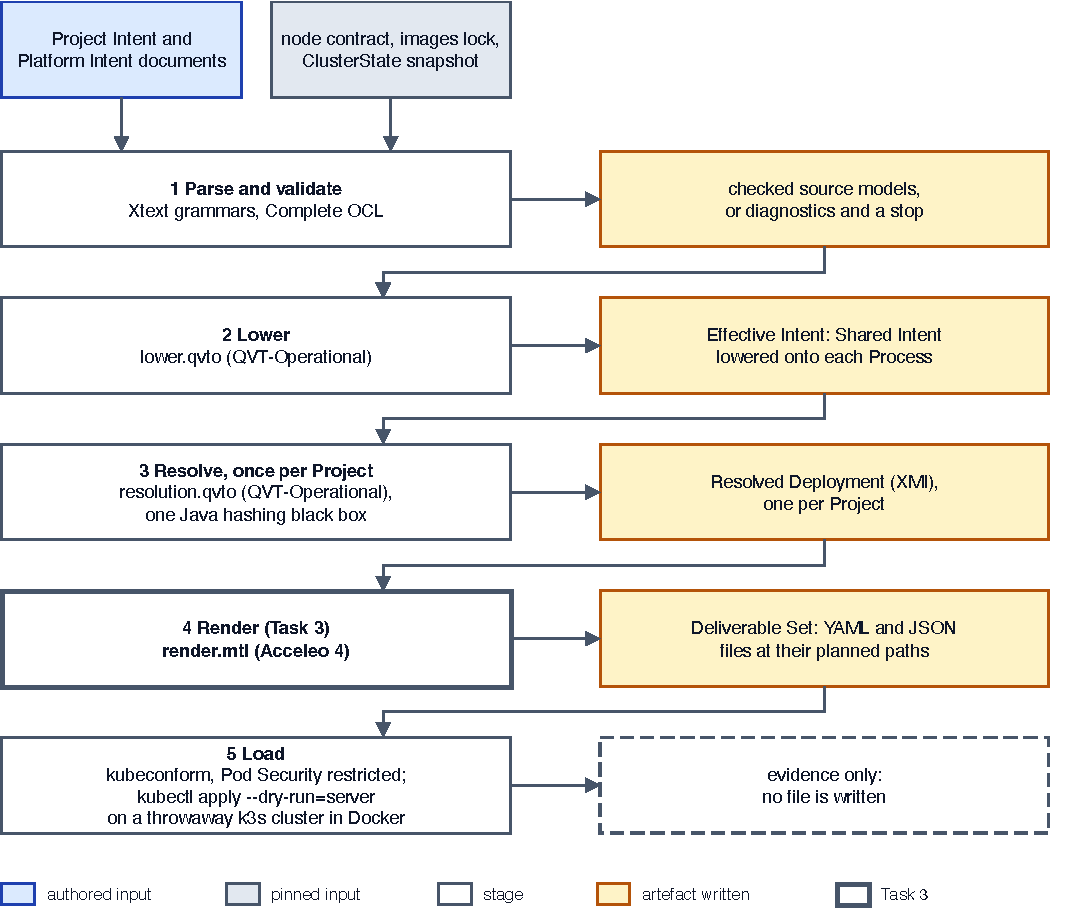
\includegraphics[width=0.82\linewidth, keepaspectratio]{Figures/pipeline}
\caption{The End-to-End Pipeline}
\label{fig:pipeline}
\end{figure}

Figure~\ref{fig:pipeline} shows five stages; Task~3 covers only rendering.
Xtext grammars and Complete OCL constraints parse and validate each document. A
QVT-Operational lowering (the flattening in Task~2) copies each Shared Intent declaration onto every
\texttt{Process} that uses it. A second QVT-Operational transformation resolves
each \texttt{Project} using the lowered models of every \texttt{Project}, the
Platform Intent and the pinned inputs. It produces one Resolved Deployment with a
path plan that assigns each Deliverable to a file. If resolution cannot derive a value,
the run stops. The Acceleo templates then run once over the set of Resolved Deployments.
Finally, the load stage checks the written files against pinned schemas, the Pod
Security \texttt{restricted} profile and a server-side dry run on a throwaway k3s
cluster (Section~\ref{sec:evaluation}).

Only resolution makes decisions; its oracle (the committed expected
models) checks them. Rendering is checked by byte comparison with the committed
\texttt{rendered} trees and by the load stage. A matching render demonstrates
correct syntax, but does not establish that the decisions were correct.

\subsection{Changes Since Task~2}
\label{sec:since-task2}

The model was refined as it was applied to production: deploying the real
estate surfaced cases the model had to express, and the changes came from those
cases. The estate pass, a third transformation over all Resolved Deployments,
was removed. The migration from the previous setup, fleet-infra with its own
DSL, was partly manual; what exists only because of it, chiefly moving data
between Instances (a Move), stems from the old deployment method rather than the
DSL, and is left out of the DSL and of this report.
Section~\ref{sec:appendix} lists each change with its reason.
% TODO(verify): confirm this summary against the appendix once it is complete.

\subsection{Roadmap}
\label{sec:roadmap}

Section~\ref{sec:alternatives} sets out the choices; Section~\ref{sec:design}
describes rendering (Figures~\ref{fig:m2t-structure} and~\ref{fig:worked-example});
Section~\ref{sec:evaluation} reports the parity and load evidence
(Figure~\ref{fig:evidence}); Section~\ref{sec:reflection} reflects on the three
tasks (Figure~\ref{fig:timeline}); Section~\ref{sec:outlook} looks beyond the
course.

% BIB: none needed in this section.
